\documentclass[
	letterpaper
]{article}

\usepackage{listings}
\lstset{language=Python,
    basicstyle=\ttfamily\small,
    stringstyle=\color{red},
    otherkeywords={0,1,2,3,4,5,6,7,8,9},
    morekeywords={TRUE,FALSE},
    deletekeywords={_data,data,frame,length,character},
    keywordstyle=\color{blue},
    commentstyle=\color{gray},
    showstringspaces=false,
}
\usepackage{array}
\usepackage{amsmath}
\usepackage{graphicx}
\usepackage{xcolor}
\usepackage{float}
\usepackage{hyperref}
\usepackage{caption}
\usepackage{subcaption}
\usepackage{xcolor}
\hypersetup{
    colorlinks,
    linkcolor={red!50!black},
    citecolor={blue!50!black},
    urlcolor={blue!80!black}
}


\title{Linear Regression built from scratch}
\date{}

\begin{document}
\maketitle
Linear regression is a supervised learning algorithm that has a deep root from statistics. 
It is one of the machine learning algorithms that looks quite simple but yet can be surprisingly useful.
In this article, we introduce the basics of a linear regression learner and build one from scratch using Python.

\section{What is regression?}
Regression is one type of supervised machine learning.

Well that does not seem to help a lot.
Let's start with one real-life example instead.
When we build a bookshelf, we have to choose plywood.
By common sense, we know if our bookshelf is wide, we need thicker or stronger plywood (assuming no other middle support is added), otherwise the bookshelf would bow because of the weights of books.
In contrast, if our bookshelf is narrow, perhaps thinner or weaker plywood would be fine.
If that is the case, then using thicker or stronger plywood would add unnecessary cost.

Here we have two groups of data: ``plywood'' and ``width of bookshelf''.
Our task is to answer this question: given our desired width of bookshelf, which plywood should we use?
If we call ``width of bookshelf'' as $x$ and ``plywood'' as $y$, then our task is simply: given x, what is y?

How do we answer this question? 
Well there are many ways to do so, one natural way is to look around existing bookshelves.
That is probably the go-to method for most people.
We just look around, find existing bookshelves, gather their width and which plywood did they use, and then determine the plywood for our new bookshelves.
The underlying rationale is that we assume our new bookshelf is similar in nature to these existing ones. 
As a result, if it has similar width as some of the existing ones, maybe we can just go ahead and use a similar plywood as those ones.

In other word, to answer the question ``given x, what is y'' , we just gather a bunch of existing $x$ and $y$.
Then we try to ``learn'' something from these existing $x$ and $y$.
Based on what we learned, we then make an educated guess of $y$ for our new $x$.
What we described here is a brief picture of supervised learning, in which the existing $x$ and $y$ are called training data, and new $x$ is called testing data.

In the world of supervised learning, if $y$ is regarded to a label or a type, such as ``pine plywood'', ``cedar plywood'', ``redwood plywood'', and so on, then this problem is called ``classification''.
In contrast, if $y$ is regarded to a continuous number, such as the thickness of a wood piece like ``0.32 inch'', ``0.44 inch'', ``0.58 inch'', and so on, then this problem is called ``regression''. (We admit this is not a great example since dimensions in traditional woodworking are usually limited to multiples of 1/8 inch, but assume we have a high-tech workshop using CNC machines to do woodworking and we can achieve any random dimension like 0.572 inch, then this is truly a regression problem.)

\section{Math expression of a linear regression}
A regression problem, like we said above, is to answer ``given $x$, what is $y$'' by looking at some existing pairs of $x$ and $y$.
In this setting, $x$ is usually called \textit{attribute} or \textit{feature}, while $y$ is usually called \textit{response} or \textit{outcome}.

Assuming we have $n$ existing pairs of $x$ and $y$, which we can written as 
\begin{equation}
X = \begin{bmatrix}
x_1 & x_2 & ... & x_n
\end{bmatrix}^T
\end{equation}
\begin{equation}
Y = \begin{bmatrix}
y_1 & y_2 & ... & y_n
\end{bmatrix}^T
\end{equation}

The task of regression is to find the relation from $X$ to $Y$.
In other words, what we need is a \textit{function approximation}.
The function from $X$ to $Y$ can be any type, but in linear regression, as the name implies, we assume this function is linear.
That is saying, we think $Y$ is approximately linear to $X$.
\begin{equation}
Y \approx wX+b
\end{equation}

In this equation, $w$ is usually called \textit{coefficient} in statistics and \textit{weight} is machine learning, while $b$ is usually called \textit{intercept} in in statistics and \textit{bias} is machine learning.
The predicted or modeled outcome $wX+b$ is often denoted as $\hat Y$.
\begin{equation}
\hat Y = wX+b
\end{equation}

In the simplest case, when $X$ only has one attribute, like out example, ``the width of bookshelf'', then $w$ is one single scalar.
This is often called \textit{simple linear regression (SLR)} in statistics.
\begin{equation}
\begin{bmatrix}\hat y_1 \\ \hat y_2 \\ ... \\ \hat y_n\end{bmatrix}
 = w\begin{bmatrix} x_1 \\  x_2 \\ ... \\ x_n\end{bmatrix}+b
\end{equation}

For most of the cases, $X$ often have more than one attribute. 
In our bookshelf example, maybe not only the width but also the height affect the choice of plywood.
For a lot of real-world problems, we have dozens or even hundreds of attributes and maybe we do not even know which attributes actually affect the outcome.
In these cases, $X$ is no longer a vector but a matrix, with rows representing different data points or instances and columns representing different data attributes or features.
This is often called \textit{multiple linear regression (MLR)} in statistics.
\begin{equation}
X =
\begin{bmatrix}
x_{1, 1} & x_{1, 2} & ... & x_{1, k} \\
x_{2, 1} & x_{2, 2} & ... & x_{2, k} \\
... & ... & ... & ... \\
x_{n, 1} & x_{n, 2} & ... & x_{n, k} \\
\end{bmatrix}
\end{equation}

In this $X$ matrix, $x_{i, j}$ represents the $j$th attribute of the $i$th data instance.
For example, $x_{1, 1}$ represents the width (1st attribute) of the 1st bookshelf and $x_{1, 2}$ represents the height (2nd attribute) of the 1st bookshelf, while $x_{2, 1}$ represents width of the 2nd bookshelf and $x_{2, 2}$ represents the height of the 2nd bookshelf.

Accordingly, $w$ is no longer a scalar but a vector with length of $k$, where $k$ is the number of attributes per instance.
\begin{equation}
\begin{bmatrix}\hat y_1 \\ \hat y_2 \\ ... \\ \hat y_n\end{bmatrix}
 = \begin{bmatrix}
x_{1, 1} & x_{1, 2} & ... & x_{1, k} \\
x_{2, 1} & x_{2, 2} & ... & x_{2, k} \\
... & ... & ... & ... \\
x_{n, 1} & x_{n, 2} & ... & x_{n, k} \\
\end{bmatrix}
\begin{bmatrix} w_1 \\  w_2 \\ ... \\ w_k\end{bmatrix}
+b
\end{equation}

For simplicity, we can also incorporate bias $b$ into this vector by adding a column of 1 as the first column of $X$ and by replacing $b$ with $w_0$.
\begin{equation}
\begin{bmatrix}\hat y_1 \\ \hat y_2 \\ ... \\ \hat y_n\end{bmatrix}
 = \begin{bmatrix}
1 & x_{1, 1} & x_{1, 2} & ... & x_{1, k} \\
1 & x_{2, 1} & x_{2, 2} & ... & x_{2, k} \\
... & ... & ... & ... & ... \\
1 & x_{n, 1} & x_{n, 2} & ... & x_{n, k} \\
\end{bmatrix}
\begin{bmatrix} w_0 \\ w_1 \\  w_2 \\ ... \\ w_k\end{bmatrix}
\end{equation}

Now we have a math representation of the regression problem.
The true outcome is $Y = [y_1, y_2, ..., y_n]$ and the predicted outcome is $\hat Y = [ \hat y_1, \hat y_2, ..., \hat y_n]$
Then our task is simply ``finding the proper $w = [w_0, w_1, w_2, ..., w_k]$ so that $\hat Y$ is as close to $Y$ as possible''.

\section{How far away is $\hat Y$ from $Y$?}
To achieve this task, the first thing we need to do is to define what do we mean by ``close to''.
In other words, we need some quantitative measure to represent how far away is $\hat Y$ from $Y$.

To define this quantitative measure, first we ask this question, what is the worst predicted $\hat Y$ a reasonable person can make?

Admittedly, we can make a lot of arbitrarily bad predictions of $\hat Y$ that is absurdly not close to $Y$ at all.
However, for a ``reasonable'' person, we can probably all agree that there is a benchmark for $\hat Y$ which is $\bar y$, the mean value of $Y$.
In our bookshelf example, this means no matter what our new bookshelf looks like, we will just use the ``average'' plywood from all existing bookshelves.
This choice might be wrong, but the point is it is not absurdly wrong.
Usually, we can use this ``wrong'' answer as a starting point for further improvement.

In math expression, guess everything as the mean of $Y$ is basically let $w_0$ be the average $Y$ and let all other $w_i$ be 0.
\begin{equation}
\begin{bmatrix}\hat y_1 \\ \hat y_2 \\ ... \\ \hat y_n\end{bmatrix}
 = \begin{bmatrix}
1 & x_{1, 1} & x_{1, 2} & ... & x_{1, k} \\
1 & x_{2, 1} & x_{2, 2} & ... & x_{2, k} \\
... & ... & ... & ... & ... \\
1 & x_{n, 1} & x_{n, 2} & ... & x_{n, k} \\
\end{bmatrix}
\begin{bmatrix} \bar y \\ 0 \\  0 \\ ... \\ 0\end{bmatrix}
=
\begin{bmatrix} \bar y \\ \bar y \\ \bar y \\ ... \\ \bar y\end{bmatrix}
\end{equation}

In this case, our true outcome is $Y = [y_1, y_2, ..., y_n]$ and our predicted outcome is $\hat Y = [\bar y, \bar y, ..., \bar y]$.
The ``distance'' between these two can then be defined as 
\begin{equation}
SS_T = \sum_{i = 1}^n (y_i - \bar y) ^2 
\end{equation}

The term $SS_T$ stands for \textit{total sum of squares}.
In some way, we can think of $SS_T$ as a lower bound benchmark of our model.
A reasonable model should at least works better than this.

Here comes our second question: how much better is our model compared to this lower bound?

In our model, we have $[w_0, w_1, w_2, ..., w_k]$ which are different from $[\bar y, 0, 0, ..., 0]$ and we somehow believe our choice is better.
How much better?
Our model predicts the outcome as $\hat Y = [\hat y_1, \hat y_2, ..., \hat y_n]$ instead of $[\bar y, \bar y, ..., \bar y]$, so the ``distance'' of our model from the lower bound is 
\begin{equation}
SS_R= \sum_{i = 1}^n (\hat y_i - \bar y) ^2 
\end{equation}

The term $SS_R$ stands for \textit{regression sum of squares}, also called \textit{explained sum of squares}. As we explained above, we can think of $SS_R$ as how much better our model is compared to the lower bound benchmark.

Nevertheless, no matter how much better our model is, we probably will not achieve perfect. 
Our third question is how far away is our model from absolutely perfect?

Our model predicts the outcome as $[\hat y_1, \hat y_2, ..., \hat y_n]$ while the prefect answer would be the true outcome which is $[y_1, y_2, ..., y_n]$.
The distance from our model to absolute perfectness is 
\begin{equation}
SS_E = \sum_{i = 1}^n (y_i - \hat y_i) ^2 
\end{equation}
The term $SS_E$ stands for \textit{error sum of squares}, also called \textit{residual sum of squares}. The smaller $SS_E$ is, the less ``error'', the closer our model is to perfectness.

For most of linear regression, it can be approved that 
\begin{equation}
SS_T = SS_R + SS_E
\end{equation}

In summary, $SS_T$ is the distance from the worst possible model to perfectness, $SS_R$ is the distance from the worst possible model to our model, and $SS_E$ is the distance from our model to perfectness.

A variable called R-Squared ($R^2$) is then defined as 
\begin{equation}
R^2 = 1 - \frac{SS_E}{SS_T} = \frac{SS_R}{SS_T}
\end{equation}

R-Squared is bound between 0 and 1. The closer to 0, the closer our model is to the worst case possible. The closer to 1, the closer our model is to perfectness.
As a result, our task is then to find $w$ that achieves the largest R-Squared.
Since $SS_T$ is a constant value of problem regardless the choice of our model, our task is then simply to minimize $SS_E$.

\section{How do we minimize $SS_E$?}
As we explained above, $SS_E$ indicates the distance between our model to perfectness, and thus we would like to minimize it.
\begin{equation}
SS_E = \sum_{i = 1}^n (y_i - \hat y_i) ^2
\end{equation}
where $\hat y_i$ is the predicted outcome from our model
\begin{equation}
\hat y_i = w_0 + x_{i, 1}w_1 + x_{i, 2}w_2 + ... + x_{i, k}w_k = \sum_{j=0} ^k x_{i, j}w_j
\end{equation}

Therefore, $SS_E$ is written as
\begin{equation}
SS_E = \sum_{i = 1}^n (y_i - \sum_{j=0} ^k x_{i, j}w_j) ^2
\end{equation}

The problem is then given $x_{i, j}$ and $y_i$, find $w_j$ that minimize $SS_E$.
This is an example of optimization problem, which can be solved by many method.
For linear regression, there is one particular effective method: \textit{gradient descend}.

The basic idea of gradient descend it to find the derivative relation between $SS_E$ and $w_j$, and gradually changing $w_j$ to the desired direction.
In other word, if increase of $w_j$ would decrease $SS_E$, we will increase $w_j$ by a little bit and see how it goes. 
In contrast, if increase of $w_j$ would increase $SS_E$,we will decrease $w_j$ by a little bit and see how it goes. 
\begin{equation}
\begin{split}
\frac{\partial SS_E}{\partial w_j} & = \frac{\partial}{\partial w_j} \sum_{i = 1}^n (y_i - \hat y_i) ^2 \\
&= \frac{\partial}{\partial w_j}\sum_{i = 1}^n (y_i - \sum_{j=0} ^k x_{i, j}w_j) ^2\\
& = \sum_{i = 1}^n \left[-2(y_i - \sum_{j=0} ^k x_{i, j}w_j)  \frac{\partial}{\partial w_j}\sum_{j=0} ^k x_{i, j}w_j \right]\\
& = \sum_{i = 1}^n \left[ -2(y_i - \sum_{j=0} ^k x_{i, j}w_j)  x_{i, j}\right] \\
& = -2\sum_{i = 1}^n\left[(y_i - \hat y_i)  x_{i, j}\right]\\
\end{split}
\end{equation}

This can also be written as 
\begin{equation}
\begin{split}
\frac{\partial SS_E}{\partial w_j} & =-2\sum_{i = 1}^n\left[(y_i - \hat y_i)  x_{i,j}\right]\\
&=-2\left[(y_1 - \hat y_1)  x_{1,j} + (y_2 - \hat y_2)  x_{2,j} + ... + (y_n - \hat y_n)  x_{n,j}\right]\\
\end{split}
\end{equation}

In matrix expression, this is
\begin{equation}
\frac{\partial SS_E}{\partial w_j} = -2 (Y - \hat Y)X
\end{equation}

We can verify this expression as 
\begin{equation}
\begin{split}
\begin{bmatrix}\frac{\partial SS_E}{\partial w_0} \\ \\ \frac{\partial SS_E}{\partial w_1} \\ \\  \frac{\partial SS_E}{\partial w_2}  \\ \\ ... \\  \\ \frac{\partial SS_E}{\partial w_k}\end{bmatrix}
& = -2 \begin{bmatrix}y_1 - \hat y_1 & y_2 - \hat y_2 & ... & y_n - \hat y_n\end{bmatrix}
\begin{bmatrix}
1 & x_{1, 1} & x_{1, 2} & ... & x_{1, k} \\
1 & x_{2, 1} & x_{2, 2} & ... & x_{2, k} \\
... & ... & ... & ... & ... \\
1 & x_{n, 1} & x_{n, 2} & ... & x_{n, k} \\
\end{bmatrix}\\
& = -2 \begin{bmatrix}
(y_1 - \hat y_1)\times 1  + (y_2 - \hat y_2) \times 1 + ... + (y_n - \hat y_n) \times 1 \\
(y_1 - \hat y_1)  x_{1,1} + (y_2 - \hat y_2)  x_{2,1} + ... + (y_n - \hat y_n)  x_{n,1}\\
(y_1 - \hat y_1)  x_{1,2} + (y_2 - \hat y_2)  x_{2,2} + ... + (y_n - \hat y_n)  x_{n,2}\\
...\\
(y_1 - \hat y_1)  x_{1,k} + (y_2 - \hat y_2)  x_{2,k} + ... + (y_n - \hat y_n)  x_{n,k}\\
\end{bmatrix}
\end{split}
\end{equation}

One we get $\frac{\partial SS_E}{\partial w_j}$, we then update $w_j$ accordingly.
If $\frac{\partial SS_E}{\partial w_j} > 0$, this indicates an increase of $w_j$ would increase $SS_E$.
Therefore we should decrease $w_j$ as the following:
\begin{equation}
w_j = w_j - \alpha \frac{\partial SS_E}{\partial w_j} 
\end{equation}
where $\alpha$ is an arbitrary coefficient to represent how much distance we would like $w_j$ to move along the desired direction.
 
In contrast, if $\frac{\partial SS_E}{\partial w_j} < 0$, this indicates an increase of $w_j$ would decrease $SS_E$.
Therefore we should increase $w_j$ as the following:
\begin{equation}
w_j = w_j - \alpha \frac{\partial SS_E}{\partial w_j} 
\end{equation}
Notice in this equation, sine $\frac{\partial SS_E}{\partial w_j} < 0$, $w_j$ minus $\frac{\partial SS_E}{\partial w_j}$ is in fact increasing $w_j$.

This is one step of gradient descend. 
To find the optimal $w$, we iterate over and over again, moving $w_j$ along the desired direction a little bit in each iteration.
Eventually, all $w_j$ is converged to its optimal value.
To check if the iteration of gradient descend is converged, we can monitor the value of $SS_E$.
If $SS_E$ does not decrease from iteration to iteration or if the decrease is too small, we can conclude the iterations are converged and there is no need to keep updating $w$.

\section{Implement gradient descend in Python}
To implement linear regression and gradient descend in Python, first we construct a class called \textit{LinearRegression}.
The variable \textit{max\_iteration} represents the allowable number of iterations such that the iteration would not run forever.
The variable \textit{tol} represents the tolerance of meaningful decrease of $SS_E$ from one iteration to the next.
If the decrease is smaller than this tolerance, then we conclude the decrease is not considerable anymore and we stop the iteration.
\begin{lstlisting}
class LinearRegression:
    def __init__(self, x, y, max_iteration=1000, tol=1e-3):
        self.max_iteration = max_iteration
        self.tol = tol
        
    def gradient_descend(self, x, y, lr=0.01):
        # Get number of instances (n) and number of attributes (d)
        n = x.shape[0]
        d = x.shape[1]

        # Initialize weights and bias with zeros
        w = np.zeros(d)

        # Initialize list to store MSE
        mse_log = []

        # Loop for gradient descent
        for i in range(self.max_iteration):
            y_pred = np.matmul(x, w)
            mse = np.mean((y - y_pred) ** 2)

            # Terminate if decrease of MSE is less than tol
            if len(mse_log) != 0 and 0<=(mse_log[-1]-mse)/mse_log[-1]<self.tol:
                break
            elif len(mse_log) != 0 and mse_log[-1] < mse:
                break
            else:
                mse_log.append(mse)

            gradient_w = -2 * np.matmul((y - y_pred), x) / n
            w -= lr * gradient_w

        return w, mse_log
\end{lstlisting}

One difference between the previous equations and the code is that we use $MS_E$ in the code rather than $SS_E$.
In the code, $MS_E$ is simply defined as $\frac{SS_E}{n}$.
As $n$ is a constant for given data, the derivative of $MS_E$ to $w$ is then
\begin{equation}
\frac{\partial MS_E}{\partial w_j} = -\frac{2}{n} (Y - \hat Y)X
\end{equation}
In the code, this is implemented as 
\begin{lstlisting}
 gradient_w = -2 * np.matmul((y - y_pred), x) / n
\end{lstlisting}

Another note is that the coefficient $\alpha$ is often called \textit{learning rate} in machine learning, which is the variable \textit{lr} in the code. But we haven't talk about how to determine learning rate yet, so our next question is what is a proper learning rate?

\section{What is a proper learning rate?}
In gradient descent, we use learning rate $\alpha$ to update weights $w$.
To successfully and effectively converge to an optimal solution, learning rate has to be proper.
Figure~\ref{fig:difflr} illustrates the effects of learning rates.
\begin{figure}[htbp]
	\centering
	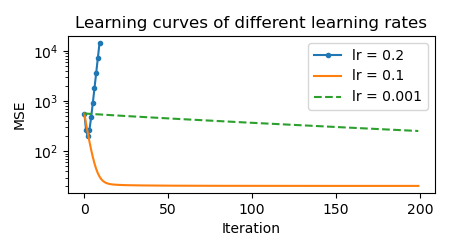
\includegraphics[width=4.2 in]{figures/diff_learning_rates.png}
	\caption{Learning curves of different learning rates}
	\label{fig:difflr}
\end{figure}

If learning rate is too small, such as the curve corresponding to learning rate of 0.001, the learning process is unnecessarily slow and the iterations do not converge within the given allowable number of iterations.
On the other hand, if learning rate is too large, then the learning process may become unstable as shown by the curve corresponding to learning rate of 0.2.
The basic assumption of partial derivative in calculus is that it only applies to a small region near that point, not applicable to regions far away from the point.
Therefore, learning rate should be kept small enough so that the movement is within that region.
In summary, learning rate needs to be in a sweet spot, not too small nor too large, like the curve corresponding to learning rate of 0.1.

In our code, we use an automatic process to tune learning rate. 
We first start with a learning rate of 0.1.
Then we try 0.01, 0.001, and so on.
We stop when the MSE achieved by a learning rate are more than 10 times larger than that of the previous learning rate.
Then the learning rate corresponding to the minimal MSE is chosen as the optima learning rate.
\begin{lstlisting}
    def tune_learning_rate(self):
        lr = 0.1
        w, mse_log = self.gradient_descend(self.x_train, self.y_train, lr=lr)
        lr_list = [lr]
        mse_list = [mse_log[-1]]

        while lr > 1e-20:
            lr *= 0.1
            w, mse_log = self.gradient_descend(self.x_train, self.y_train, lr=lr)
            # if mse is 10 times larger than previous iteration, stop
            if mse_log[-1] > 10 * mse_list[-1]:
                break
            lr_list.append(lr)
            mse_list.append(mse_log[-1])

        opt_lr = lr_list[mse_list.index(min(mse_list))]

        return opt_lr
\end{lstlisting}

\section{Scale data before training}
For linear regression, it is not required to use scaled data.
However, our code still scales and centers data before training.
The first reason is that this help our autonomous tuning of learning rate.
If the data is not scaled, staring from a learning rate of 0.1 maybe far away from the actual reasonable learning rate.
The second reason is that several advanced methods, which are based on linear regression, such as LASSO, rigid regression, and elastic net, all require the data to be scaled.
To use our code as the foundation of these methods in the further, we apply data scaling and centering in our code.
\begin{lstlisting}
class LinearRegression:
    def __init__(self, x, y, max_iteration=1000, tol=1e-3):
        self.max_iteration = max_iteration
        self.tol = tol
        
        self.x_raw = x
        self.mu = np.mean(x, axis=0)
        self.sigma = np.std(x, axis=0)
        self.x_train = self.standard_transform(x)
        self.y_train = y
        self.weights = None
        
    def standard_transform(self, x):
        scaled_x = (x - self.mu) / self.sigma
        scaled_x = np.insert(scaled_x, 0, np.ones(scaled_x.shape[0]), axis=1)
        return scaled_x
\end{lstlisting}

In this function, besides scaling and centering, we also insert a column of 1 as the first column of $X$ so that we have a single $w$ vector without using an additional variable of $b$ for bias.

\section{API of the learner}
We use the following API to train and utilize the learner.
\begin{lstlisting}
    def fit(self, lr=None):
        if lr is None:
            lr = self.tune_learning_rate()
        w, mse_log = self.gradient_descend(self.x_train, self.y_train, lr=lr)
        self.weights = w
    
    def predict(self, x):
        x_test = self.standard_transform(x)
        return np.matmul(x_test, self.weights)
\end{lstlisting}

Using this API, for given training and testing data sets, a learner can be built and trained using the following code:
\begin{lstlisting}
learner = LinearRegression(x_train, y_train, plot=plot, verbose=True)
learner.fit()
\end{lstlisting}
To validate the learner by training data set, we can get predicted y of training x.
\begin{lstlisting}
y_pred_train = learner.predict(x_train)
\end{lstlisting}
To utilize the learning on testing data set, we can get predicted y of testing x.
\begin{lstlisting}
y_pred_test = learner.predict(x_test)
\end{lstlisting}

\section{Example using \textit{diamonds} data set}
We use \textit{diamonds} data set from \textit{R} package \textit{yarrr} as an example to run our learner.
This data set has 150 data instances and 3 attributes: weight, clarity scale, and color scale.
The outcome is the value of the diamond.
A part of the data set is previewed in the following table:
\begin{table}[htbp]
	\small 
	\centering 
		\caption{Preview of \textit{diamonds} data set}
		\label{table:diamonds}
	\begin{tabular}{r r r|r}
		Weight & Clarity & Color & Value \\
9.35	&		0.88	&		4		&	  182.5\\
11.10	&   1.05	&		5		&  191.2\\
8.65	&		0.85	&		6		&  175.7\\
10.43	&		1.15	& 	5		&  195.2\\
10.62	&		0.92	&		5		&  181.6\\
12.35	&		0.44	&		4		&  182.9\\
11.24	&		1.09	& 	6		&  195.9\\
9.77	&		1.43	&		4		&  188.6\\
11.83	& 	0.95	&		6		&  190.3\\
9.55	&		1.05	&		5		&  190.7\\
	\end{tabular}
 \end{table}
 
For this example, we use \textit{train\_test\_split} function from \textit{sklearn.model\_selection} to split the data set into training and testing.
\begin{lstlisting}
df = pd.read_csv('data/diamonds.csv', sep=' ')
df = df.to_numpy()
x = df[:, 0:-1]
y = df[:, -1]
x_train, x_test, y_train, y_test = train_test_split(x, y)
learner = LinearRegression(x_train, y_train, plot=plot)
learner.fit()
y_pred_train = learner.predict(x_train)
y_pred_test = learner.predict(x_test)
\end{lstlisting}

The autonomous tuning of learning rates is shown in Figure~\ref{fig:tune_lr}.
For this data set, learning rate of 0.1 seems to be the optimal choice as it achieved the minimal MSE and uses the smallest number of iterations.
\begin{figure}[htbp]
	\centering
	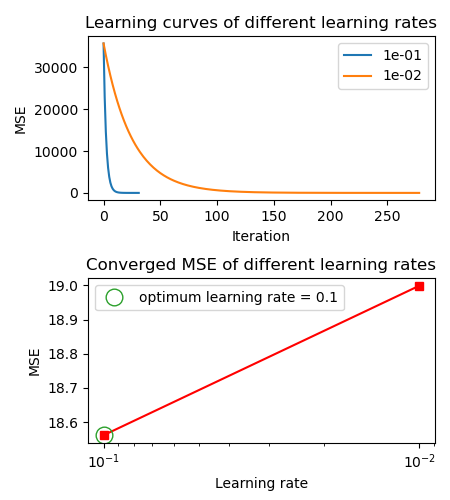
\includegraphics[width=3.5 in]{figures/tune_learning_rates.png}
	\caption{Tune of learning rate for \textit{diamonds} data set}
	\label{fig:tune_lr}
\end{figure}

The results of the model can be visualized by plotting predicted values versus true values using the following code:
\begin{lstlisting}
fig, axes = plt.subplots(1, 2)
axes[0].plot(y_train, y_pred_train, marker='o', markersize=4, 
             linestyle='None', color='#1f77b4')
axes[0].axline((np.mean(y_train), np.mean(y_train)), slope=1., color='red')
axes[1].plot(y_test, y_pred_test, marker='o', markersize=4, 
             linestyle='None', color='#2ca02c')
axes[1].axline((np.mean(y_test), np.mean(y_test)), slope=1., color='red')
plt.show()
\end{lstlisting}

For the \textit{diamonds} data set, the training and testing results as visualized in Figure~\ref{fig:res_diamonds}.
The closer our predictions to the true values, the closer these plotted points to the red diagonal line.
As we can see in the figure, the points in training and testing plots generally lay along the diagonal line. 
\begin{figure}[htbp]
	\centering
	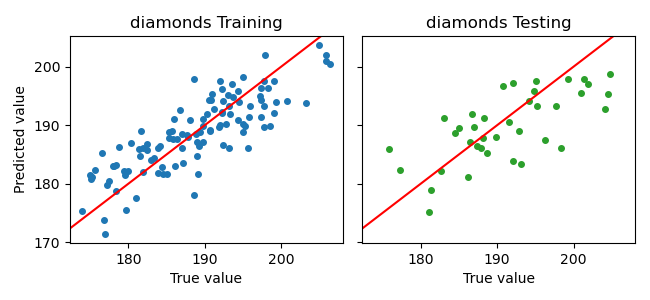
\includegraphics[width=4.2 in]{figures/res_diamonds.png}
	\caption{Visualization of predicted values versus true values for \textit{diamonds} data set}
	\label{fig:res_diamonds}
\end{figure}

\section{How do we interpolate the learning?}
Now we have finished our linear regression on this \textit{diamonds} data set. 
Imagine we need to give an elevator pitch to business partners or policy makers, what should we present?
One of the most important outputs of linear regression is the weights of each data attributes, which give us insights onto the relations between attributes and outcome.

As we did gradient descent on scaled data, out weights also corresponds to the scaled data.
To relate the weights back to original data, we need to do some calculation to derive the weights for uncalled data.
\begin{lstlisting}
def get_unscaled_weights(self):
    unscaled_wights = self.weights[1:] / self.sigma
    unscaled_intercept = self.weights[0]-np.sum(self.weights[1:]*self.mu/self.sigma)
    unscaled_wights = np.insert(unscaled_wights, 0, unscaled_intercept)
    return unscaled_wights
\end{lstlisting}

Using this function, we obtain the weights for each attributes in the \textit{diamonds} data set.
As we explained before, the data outcome, which is the value of diamonds, can be approximated using a linear combination of weights and data attributes:
\begin{equation}
\begin{split}
\text{diamond value} = &148.37+ 2.35 (\text{weight}) + 20.18(\text{clarity})-0.58(\text{color}) \\
\end{split}
\end{equation}

For this simple data set, we learn from the weights that the more the weights, the more the value, which seems reasonable.
We also learn that the higher the clarity grade, the more the value, which also makes sense as people prefer diamonds with little inclusion or blemish.
For color, the lower the color scale, the more the value, which probably indicates people prefer colorless diamonds.

\section{How confident are we?}
In our elevator pitch, we present the linear equation above and we talk about the relation between price and weight, clarity, or color.
However, there is one an important question: how sure are we?
In more technical words, in statistics, is our model significant enough?

To answer this question, we can perform a \textit{significance test}.
We still use $n$ as the number of data instances and $k$ as the number of data attributes.
We already talked about $SS_T$, $SS_R$, and $SS_E$, which are total sum of square, regression (explained) sum of square, and error (residual) sum of square, respectively.
One indicator regarding how well is out model is R-Squared which is already covered previously
\begin{equation}
R^2 = 1 - \frac{SS_E}{SS_T} = \frac{SS_R}{SS_T}
\end{equation}

One drawback of using R-Squared is that it is compromised by increasing number of attributes.
If the number of attributes is huge, then we can find $w$ that generate a very small $SS_E$ and thus a very large R-Squared.
However, this does not necessarily indicate that our model is perfect.
As there are so many random effects in these huge number of attributes, the model captured almost all of these random effect to achieve a high R-Squared.
In machine learning, this is an example of \textit{overfitting}.
To overcome this, we introduce an adjusted version of R-Squared to address this.

To determine adjusted R-Square, we first define the corresponding mean of sum of squares.
\begin{equation}
MS_T = \frac{SS_T}{n-1}
\end{equation}
\begin{equation}
MS_R = \frac{SS_T}{k}
\end{equation}
\begin{equation}
MS_E = \frac{SS_E}{n-(k+1)}
\end{equation}

Then the adjusted R-Squared is defined as
\begin{equation}
R_{\text{adjusted}}^2 = 1 - \frac{MS_E}{MS_T}
\end{equation}

The relation between R-Squared and adjusted R-Squared can be derived.
\begin{equation}
\begin{split}
R_{\text{adjusted}}^2 &= 1 - \frac{MS_E}{MS_T}\\
& =  1 - \frac{\frac{SS_E}{n-(k+1)}}{\frac{SS_T}{n-1}}\\
& = 1 - \frac{n-1}{n-(k+1)} \frac{SS_E}{SS_T}\\
& = 1 - \frac{n-1}{n-(k+1)} (1-R^2)
\end{split}
\end{equation}

We can see that adjusted R-Squared decreases as $k$ increases.
In some sense, we can say using adjusted R-Squared encourages models with less data attributes.
In other words, if two models achieve same R-Squared, but one with significantly smaller number of attributes, then adjusted R-Squared tells us this model is better than the other one.

R-Squared and adjusted R-Squared can be calculated using the following code.
\begin{lstlisting}
y = self.y_train
y_pred = np.matmul(self.x_train, self.weights)

n = self.x_train.shape[0]
k = self.x_train.shape[1] - 1

ss_total = np.sum((y - np.mean(y)) ** 2)
ms_total = ss_total / (n - 1)

ss_regression = np.sum((y_pred - np.mean(y)) ** 2)
ms_regression = ss_regression / k

ss_error = np.sum((y - y_pred) ** 2)
ms_error = ss_error / (n - k - 1)

r_square = 1 - ss_error / ss_total
adj_r_square = 1 - ms_error / ms_total
\end{lstlisting}

In our \textit{diamonds} example, the R-Squared turns out to be 60.38\% and the adjusted R-Squared turns out to be 59.28\%.

Now we are ready to perform the significance test.
For linear regression, we usually use a F-test to assess the significance.
The \textit{F-statistic} is defines as the ratio between the \textit{explained} variances to \textit{unexplained} variances.
\begin{equation}
F = \frac{MS_R}{MS_E}
\end{equation}

Using this \textit{F-statistic}, we can then determine the corresponding $P$ value.
To do that, first we need to determine the degree of freedom (dof) of the F-distribution.
In linear regression, the first dof is $k$ and the second dof is $n - (k+1)$.
In our \textit{diamonds} example, we are looking at first dof of 3 and second dof of 108.
The F-distribution and the corresponding survival function is plotted in the Figure~\ref{fig:f-test}.
\begin{figure}[htbp]
	\centering
	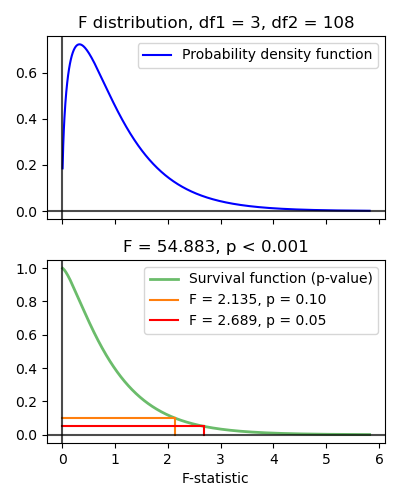
\includegraphics[width=3.2 in]{figures/f-test.png}
	\caption{F-test of linear regression on \textit{diamonds} data set}
	\label{fig:f-test}
\end{figure}

When $F=2.689$, the area under the probability density curve on the right side of 2.689 is 0.05, indicating a $F$ value of 2.689 corresponds to a $P$ value of 0.05.
Similarly, the area under the probability density curve on the right side of 2.135 is 0.10, indicating a corresponding $P$ value of 0.10.
In our \textit{diamonds} example, our $F$ turns out to be 54.883, which is way on the right of our plot.
As a result, the P-value is extremely small.

P-value has strict definitions in statistics which we will not go into details today.
What we need to know is that P-value indicates the probability that the reason why our model performs this well is purely by luck.
In this case, this probability is very low, definitely smaller than 0.001.
In statistics, 0.05 is usually used as the threshold.
As a result, we conclude that this is not caused by pure luck, and thus, our model is at least somewhat ``meaningful'', which is called ``significant'' in statistics.

\section{Are every attribute relevant?}
































\end{document}